	Comme nous l'avons dit précédemment, pour réaliser le dashboard il a été décidé que la stack ELK serait utilisée. J'ai donc, dans un premier temps, du me former à l'utilisation de cette dernière qui est constituée de trois produits de la société Elastic que sont Elasticsearch, Logstash et Kibana. Son objectif premier est de stocker, d'analyse et de lire les logs générer par un projet tel qu'une API REST dans l'optique de faire du monitoring, de suivre l'activité d'un service ou de prévenir des dysfonctionnements. Nous allons maintenant décrire en quoi chacun des outils est intervenu dans le processus de réalisation du dashboard. Pour cela, il est possible de se référer à la figure \ref{elk} afin de pouvoir situer chaque composant.

	\subsubsection{Elasticsearch}
	La quantité de logs générés par une application de cette ampleur peut rapidement devenir très conséquente et de nombreuses problématiques sont alors soulevées concernant le stockages des messages importants, leur recherche ou leur analyse. Les bases données relationnelles classiques ont montré leurs limites concernant le travail avec de tels volumes de données sur le long terme que ce soit pour le stockage ou les temps de réponse lors d'une recherche, et ce malgré des requêtes bien construites avec des jointures judicieuses entre les tables. Elasticsearch a pour objectif de répondre à cette problématique. \\
	
	Il s'agit d'un moteur d'indexation, de stockage et de recherche de données développé en Java basé sur \textit{Lucene}, une bibliothèque d'indexation et de recherche de texte créée par la fondation Apache. Son principal atout est qu'il permet de stocker de large volume de données tout en permettant aux utilisateurs d'effectuer des recherches en temps réel. Les données sont stockées sous la forme de \textit{document}. Il s'agit d'une unité basique d'information qui peut être indexée. Les index sont des collections de documents possédant des caractéristiques similaires. Les index peuvent aussi posséder un type afin de les diviser en plusieurs parties "logiques". On peut, par exemple, créer un index \textit{api-microservices-2017.07} avec un type \textit{log}. 
	
	On pourra alors récupérer le document d'id 1 avec la requête suivante :	

\begin{lstlisting}[language=json]
 GET api-microservices-2017.07/log/1?pretty
 \end{lstlisting}
	
	La réponse contiendrait ledit document avec les champs définis par nos soins (ici timestamp, logLevel, service et message) :
	
\begin{lstlisting}[language=json]
{
 "_index": "api-microservices-2017.07",
 "_type": "log",
 "_id": "1",
 "_version": 1,
 "found": true,
 "_source" : {
  "timestamp": "2017-07-07T14:15:45",
  "logLevel": "INFO",
  "service": "account-service"
  "message": "elasticsearch example"
 }
}
	\end{lstlisting}
	 
	 Dans notre cas, Elasticsearch est utilisé comme support de stockage qui sera par la suite interrogé par Kibana. Cependant, il peut tout à fait être interroger depuis une API, c'est pourquoi il ne dispose pas de client dédié.
	
	\subsubsection{Logstash}
	Logstash est un \textit{ETL} ou \textit{Extract-transform-load}. Cela désigne les outils capable de synchroniser des volumes de données massif depuis une source précise vers une autre. Ainsi, Logstash agit un peu à la manière d'un pipeline capable de prendre un grand nombre de messages en entrée depuis plusieurs sources pour les traiter, effectuer des transformations ou encore les filtrer avant de les renvoyer vers un support de stockage. Le schéma figure \ref{logstash} explicite son principe de fonctionnement. La liste des technologies mentionnées dans celui-ci n'est pas exhaustive, il s'agit purement d'exemples de ce qu'il est possible de faire à titre démonstratif. \\
	
	\begin{figure}[h!]
		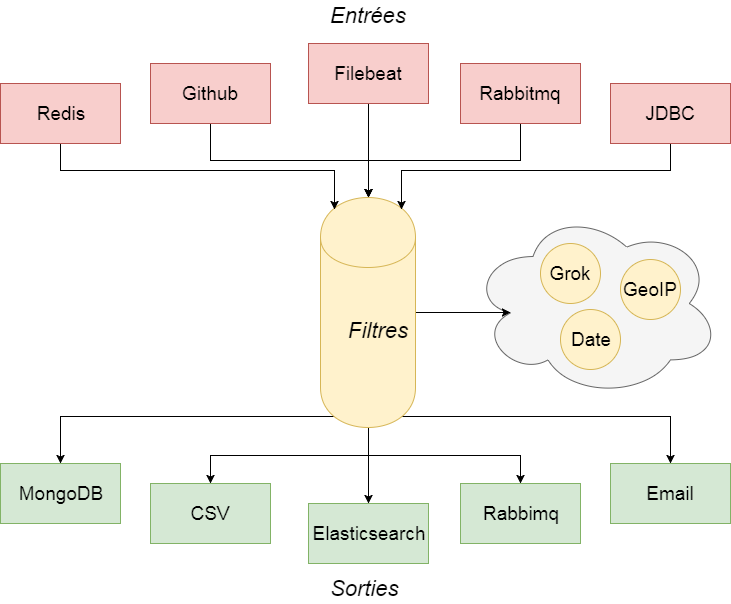
\includegraphics[scale=0.4]{images/travailNeuflizeOBC/dashboard/logstash.png}
		\centering
		\caption{Logstash}
		\label{logstash}
	\end{figure}
	
	Logstash accepte en entrée un nombre impressionnant de formats différents comme tout ce qui est représenté sous forme de chaîne de caractères mais aussi les événements issus de sources différentes et ce de manière simultanée. Dans notre cas, logstash prendra en entrée des fichiers logs fournit par Filebeat dont nous parlerons plus en détails peu après. Ces logs auront été générés au préalable par l'API microservices à l'aide de \textit{Logback}. \\
	
	Une fois les données acquises, celles-ci sont analysées puis transformer par les filtres de Logstash. Il est ainsi possible d'ajouter, modifier ou supprimer de l'information, extraire des valeurs depuis des messages, analyser des événement et bien d'autres. Le filtre le plus puissant mis a disposition par Logstash est \textit{Grok} que nous utiliserons ici et qui permet de transformer dynamiquement des données non structurées en données structurées en découpant une ligne de log en un ensemble de champs prédéfinis. Nous pourrons donc utiliser ce filtre afin de structurer les informations de telle manière qu'elles soient facilement exploitable par Kibana. Par exemple, la ligne de log suivante :
	
\begin{lstlisting}[language=json]
 [2017-07-07T14:15:45] [INFO] [account-service] - elasticsearch example
\end{lstlisting}
	
	peut être transformer sous la forme du document structuré montré en exemple plus haut à l'aide d'un filtre adéquat définissant les champs (comme timestamp ou loglevel). \\
	
	Enfin, une fois les données formatées, il est possible de les envoyer vers la destinaiton de notre choix, et là encore Logstash offre la possibilité de transmettre les données vers un grand nombre de sources différentes. Il sera bien évidemment ici connecté à Elasticsearch et permettra donc de stocker les logs de manière structurée et indexée au sein de la base de données. En outre, il offre une grande flexibilité puisque chacune des entrées/sorties ou mêmes les filtres sont implémentés sous la forme de plugin. Par ailleurs, la société Elastic a mis à disposition une API permettant de faciliter le développement de ces plugins, ce qui permet d'ajouter de nombreuses nouvelles possibilités à Logstash.
	
	\subsubsection{Kibana}
	Avec les outils précédent nous avons de quoi stocker nos logs, les analyser, les transformer pour structurer les informations qu'ils contiennent et rechercher ce que nous souhaitons parmis eux à l'aide de requêtes Elasticsearch. Cependant, cela n'est absolument pas "user friendly" et nécessite des connaissances techniques ce qui ne suffit pas à satisfaire le besoin client. Kibana permet palier cette faiblesse en nous fournissant une interface nous permettant de choisir la mise en forme de nos données. Celui-ci permet de construire des graphiques, nommés \textit{visualisations}, tels que des histogrammes, des camemberts ou encore des tableaux. Ensuite, Kibana permet de choisir une plage de date pour ne traiter que les données situées dans cette dernière. Une fois le dashboard et les visualisations créés, il suffit de changer le temps et tous les graphiques s'actualiseront automatiquement ce qui permet de facilement retrouver des informations. Par exemple, il suffit d'un simple clic pour connaitre le nombre de connexion qu'il y a eu hier, le mois dernier ou entre le 23 juillet et le 15 août. De plus, Kibana vient avec une nouvelle composante nommée \textit{Timelion} permettant d'effectuer des analyses chronologiques approfondies. \\
	
	Ici, Kibana alimentera les visualisations avec les données stockées dans la base d'Elasticsearch et sera l'unique interface homme machine utilisée. En effet, il offre une console développeur permettant de faciliter la construction des requêtes Elasticsearch et permet de visualiser les données stockées en base à l'aide une option \textit{discovery} affichant pour chaque ligne de log brute les champs structurés définis dans logstash.
	
	\subsubsection{Filebeat}	
	Elastic a mis à notre disposition, en plus de la stack ELK, des agents de transfert nommés les \textit{Beats}. Il en existe pour tout type de données mais dans notre cas nous utiliserons Filebeat conçu spécialement pour le transfert des logs et fichiers. Celui-ci permet de collecter l'ensemble des logs, qu'importe où ils se trouvent, pour les envoyer ensuite à Logstash. Il est possible de le configurer pour qu'il ne transfert pas les fichiers de logs entiers mais seulement les lignes qui nous intéressent. Celui-ci ne nécessite aucune intervention humaine une fois qu'il est mis en place, à chaque ligne de log générée il en est informé et effectue le transfert automatiquement. En outre, si Logstash est occupé et possède déjà un gros volume de données à traiter, Filebeat en sera également informé et pourra ralentir son flux d'envoi afin d'éviter tout problème de congestion.

	\subsubsection{Les intéractions en résumé}
	Toutes les intéractions entre les différents composants sont résumées sur le schéma figure \ref{elk}. Pour commencer, les logs sont générés par l'API microservices grâce à Logback qui permet de configurer quelle ligne ira dans quel fichier et où ces derniers seront créés. Dès que des lignes de logs sont générées, Filebeat est averti et va donc lire le fichier de logs concerné, détecter les nouvelles lignes puis les envoie à Logstash si elles remplissent les critères. Ce dernier récupère ces lignes non structurées en entrée et agit comme un pipeline qui produira en sortie des données structurés à l'aide de champs prédéfinis. Ensuite, Elasticsearch reçoit ces données de la part de Logstash, les indexe puis les stocke en base de données. Enfin, Kibana interroge Elasticsearch à l'aide de requêtes en fonction du temps sélectionné pour alimenter les visualisations créées au sein du dashboard. 
	
\begin{figure}[h!]
	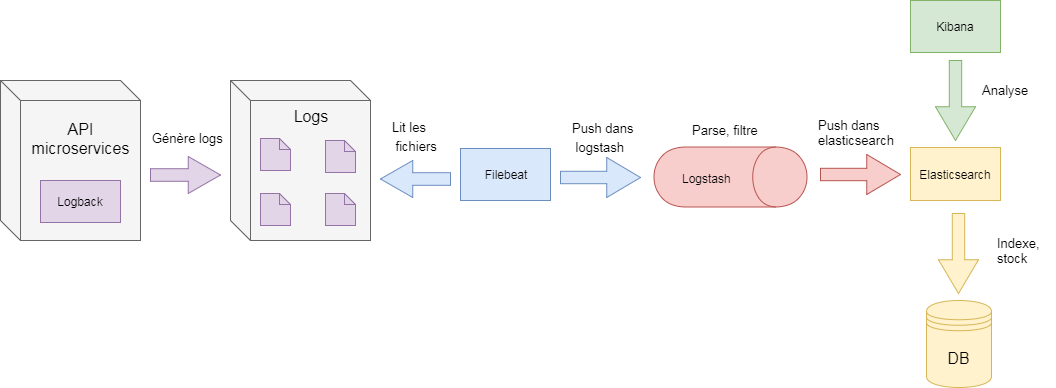
\includegraphics[scale=0.5]{images/travailNeuflizeOBC/dashboard/elk.png}
	\centering
	\caption{Intéractions au sein de la stack ELK}
	\label{elk}
\end{figure}